\documentclass[aspectratio=169]{beamer}

% --- Packages ---
\usepackage[utf8]{inputenc}
\usepackage{graphicx}
\usepackage{pgfpages}
\usepackage{hyperref}
\usepackage{booktabs}
\usepackage{amssymb}
\usepackage{amsmath}
\usepackage{siunitx}
\usepackage{microtype}
\usepackage{float}
\usepackage{tikz}
\usetikzlibrary{positioning}

% --- Theme Selection ---
\usetheme{Boadilla}
\usecolortheme{seahorse}

% --- Custom Styling ---
\setbeamertemplate{navigation symbols}{} % Remove navigation symbols
\setbeamertemplate{caption}[numbered] % Numbered captions
\setbeamertemplate{bibliography item}[text] % Numbered bibliography [1]
\setbeamertemplate{sections/subsections in toc}[default] % Unnumbered Table of Contents (uses our Part X labels cleanly)

% --- Custom Colors & Formatting ---
\definecolor{BMEblue}{RGB}{0,91,153}
\setbeamercolor{structure}{fg=BMEblue}
\setbeamercolor{title}{fg=BMEblue,bg=white}
\setbeamercolor{frametitle}{fg=BMEblue,bg=white}

% --- Metadata ---
\title[Characterization of High-Tc DC SQUID]{Characterization of a High-Temperature DC SQUID}
\subtitle{V-I Traces, Magnetometry, and Shapiro Step Detection}
\author[Jaca, Tallosy]{Gregorio Jaca (U8L9B9), Peter Tallosy (K14WR1)}
\institute[BME]{Budapest University of Technology and Economics \\ Department of Physics \\ Nanoelectronics Laboratory}
\date{May 2026}

\begin{document}

% ---------------------------------------------------------------------
% Slide 1: Title Page
% ---------------------------------------------------------------------
\begin{frame}[plain]
    \titlepage
\end{frame}

% ---------------------------------------------------------------------
% Slide 2: Outline
% ---------------------------------------------------------------------
\begin{frame}{Outline}
    \tableofcontents
\end{frame}

% =====================================================================
% SECTION 1: INTRODUCTION & MOTIVATION
% =====================================================================
\section{Part 1: Motivation and Theoretical Foundation}
\begin{frame}[plain,noframenumbering]
    \centering
    \large\bfseries\color{BMEblue}
    Part 1: Motivation and Theoretical Foundation
\end{frame}

% ---------------------------------------------------------------------
% Slide 3: Motivation
% ---------------------------------------------------------------------
\begin{frame}{Motivation: Frontier of High-Sensitivity Quantum Sensing}
    \begin{columns}
        \column{0.55\textwidth}
        \textbf{Why Superconducting Quantum Interference?} \\
        \vspace{0.1cm}
        SQUIDs exploit macroscopic quantum coherence to resolve magnetic flux below a single quantum $\Phi_0$, making them the ultimate flux-to-voltage transducers.
        
        \vspace{0.2cm}
        \textbf{Key Applications in Frontier Physics} \\
        \vspace{0.1cm}
        \begin{itemize}
            \item \textbf{Biomedical MEG}: Mapping brain activity [Hämäläinen 1993].
            \item \textbf{Scanning SQUID (SOT)}: Imaging nano-spins and thermal dissipation [Vasyukov 2013, Halbertal 2016].
            \item \textbf{Metrology}: Phase-locked Josephson voltage standards.
        \end{itemize}

        \column{0.45\textwidth}
        \centering
        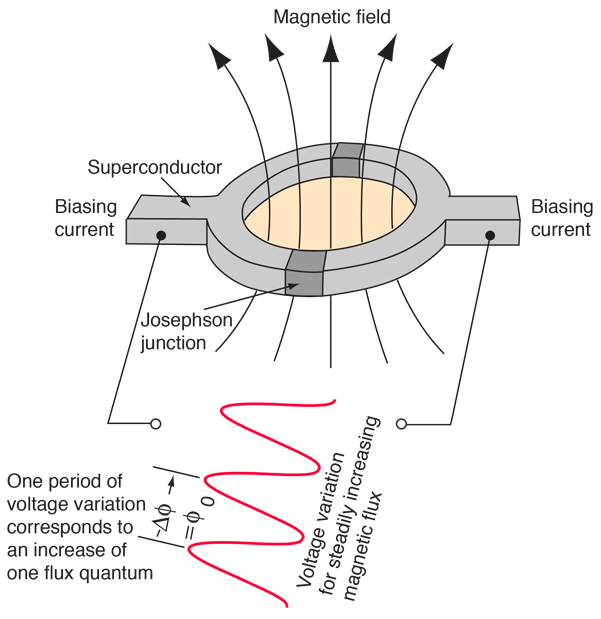
\includegraphics[height=0.52\textheight,keepaspectratio]{squide.png} \\
        \vspace{0.1cm}
        \scriptsize SQUID loop and phase modulation schematic
    \end{columns}
\end{frame}

% ---------------------------------------------------------------------
% Slide 4: Theoretical Foundation - The Josephson Effect
% ---------------------------------------------------------------------
\begin{frame}{Theoretical Foundation: Josephson Effect}
    \begin{columns}
        \column{0.55\textwidth}
        \textbf{Macroscopic Quantum Wave Function} \\
        Condensate is modeled by $\Psi = \sqrt{\rho} e^{i\phi}$. Two weak-link superconductors separated by an insulating barrier exhibit phase difference $\delta = \phi_1 - \phi_2$ [Sólyom Vol 2, Feynman Lectures].
        
        \vspace{0.2cm}
        \textbf{Josephson Equations} \\
        \begin{itemize}
            \item \textbf{DC Relation}: Dissipationless supercurrent
            \begin{equation}
                I = I_c \sin\delta
            \end{equation}
            \item \textbf{AC Relation}: Phase evolution under voltage bias $V$
            \begin{equation}
                \dot{\delta} = \frac{2eV}{\hbar} = \frac{2\pi}{\Phi_0} V
            \end{equation}
        \end{itemize}
        
        \column{0.45\textwidth}
        \textbf{Josephson Non-Linear Inductance} \\
        Differentiating current yields a phase-dependent inductance:
        \begin{equation}
            L_J(\delta) = \frac{\Phi_0}{2\pi I_c \cos\delta}
        \end{equation}
        This non-linear behavior makes JJs the primary building blocks of qubits, preventing harmonic over-excitation [Makk Lecture Notes].
    \end{columns}
\end{frame}

% ---------------------------------------------------------------------
% Slide 5: Theoretical Foundation - The DC SQUID
% ---------------------------------------------------------------------
\begin{frame}{Theoretical Foundation: DC SQUID}
    \begin{columns}
        \column{0.40\textwidth}
        \textbf{Macroscopic Interference} \\
        \small Two parallel JJs enclosing a loop enforce the phase constraint:
        \begin{equation}
            \delta_2 - \delta_1 = \frac{2e}{\hbar}\oint \vec{A}\cdot d\vec{r} = 2\pi\frac{\Phi_{\text{ext}}}{\Phi_0}
        \end{equation}
        
        \vspace{0.1cm}
        \textbf{Current Modulation} \\
        \small Supercurrent interference yields:
        \begin{equation}
            I_{c,\text{SQUID}} = 2I_c \left|\cos\left(\pi\frac{\Phi_{\text{ext}}}{\Phi_0}\right)\right|
        \end{equation}
        
        \column{0.35\textwidth}
        \textbf{Voltage Transduction} \\
        \small Constant current bias $I_{\text{bias}} > 2I_c$ yields a flux-dependent voltage:
        \begin{equation}
            V(\Phi) = \frac{R}{2} \sqrt{I_{\text{bias}}^2 - I_{c,\text{SQUID}}^2(\Phi)}
        \end{equation}
        \small The SQUID translates external magnetic fields into microvolts, enabling sub-quantum magnetometry [Granata et al. 2016].
        
        \column{0.25\textwidth}
        \centering
        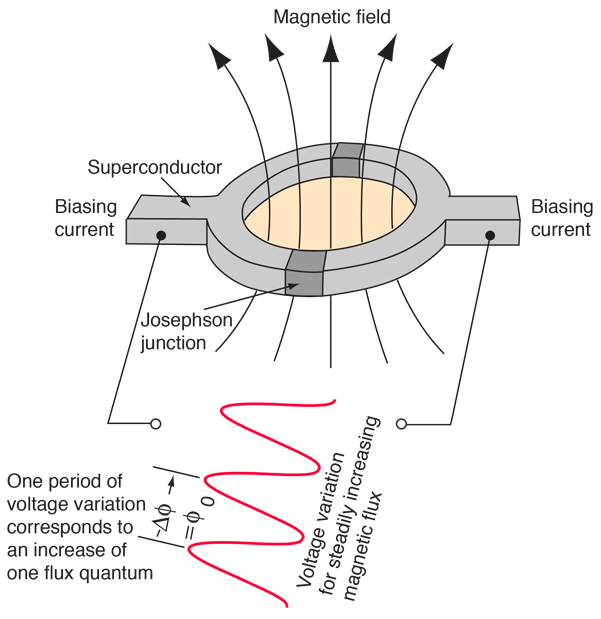
\includegraphics[width=\textwidth,keepaspectratio]{squide.png} \\
        \vspace{0.05cm}
        \scriptsize SQUID schematic and modulation
    \end{columns}
\end{frame}

% =====================================================================
% SECTION 2: EXPERIMENTAL SETUP
% =====================================================================
\section{Part 2: Cryogenic Experimental Setup and Noise Mitigation}
\begin{frame}[plain,noframenumbering]
    \centering
    \large\bfseries\color{BMEblue}
    Part 2: Cryogenic Experimental Setup and Noise Mitigation
\end{frame}

% ---------------------------------------------------------------------
% Slide 6: Experimental Setup
% ---------------------------------------------------------------------
\begin{frame}{Cryogenic Experimental Setup}
    \begin{columns}
        \column{0.55\textwidth}
        \textbf{High-Tc SQUID Setup} \\
        \begin{itemize}
            \item \textbf{YBCO SQUID}: grain-boundary bicrystal device cooled in liquid nitrogen ($T = 77\text{ K}$) [SQUID.md].
            \item \textbf{Current Bias}: Waveform Generator driven through a $10\text{ k}\Omega$ series resistor ($R_{\text{series}} \gg R_N$).
            \item \textbf{Voltage Sensing}: SQUID voltage amplified $1000\times$ by low-noise differential op-amp and filtered.
            \item \textbf{RF Coupling}: HP 8620C sweep oscillator delivering microwave signals (8--12 GHz) via SMA line.
        \end{itemize}

        \column{0.45\textwidth}
        \centering
        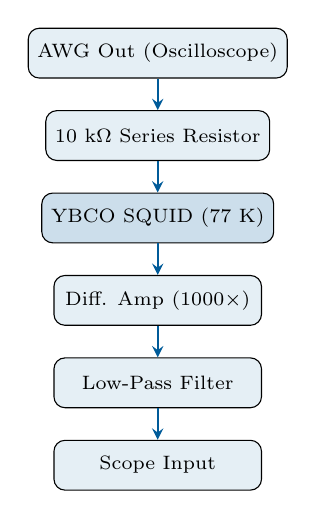
\begin{tikzpicture}[
            box/.style={draw, rectangle, fill=BMEblue!10, text centered, minimum height=1.8em, minimum width=7.5em, rounded corners, font=\scriptsize},
            arrow/.style={-stealth, thick, BMEblue}
        ]
            \node (awg) [box] {AWG Out (Oscilloscope)};
            \node (res) [box, below=0.4cm of awg] {$10\text{ k}\Omega$ Series Resistor};
            \node (squid) [box, below=0.4cm of res, fill=BMEblue!20] {YBCO SQUID (77 K)};
            \node (amp) [box, below=0.4cm of squid] {Diff. Amp ($1000\times$)};
            \node (lpf) [box, below=0.4cm of amp] {Low-Pass Filter};
            \node (scope) [box, below=0.4cm of lpf] {Scope Input};
            
            \draw [arrow] (awg) -- (res);
            \draw [arrow] (res) -- (squid);
            \draw [arrow] (squid) -- (amp);
            \draw [arrow] (amp) -- (lpf);
            \draw [arrow] (lpf) -- (scope);
        \end{tikzpicture} \\
        \vspace{0.1cm}
        \scriptsize Cryogenic measurement circuit schematic
    \end{columns}
\end{frame}

% ---------------------------------------------------------------------
% Slide 7: Noise Mitigation & Parametric Derivatives
% ---------------------------------------------------------------------
\begin{frame}{Noise Mitigation and Parametric Derivatives}
    \begin{columns}
        \column{0.55\textwidth}
        \textbf{Noise Reduction} \\
        Cryogenic thermal noise requires hardware averaging ($4\times$/$16\times$) on the oscilloscope to suppress random fluctuations.
        
        \vspace{0.2cm}
        \textbf{Parametric derivative methodology} \\
        Numerical differentiation $dV/dI$ introduces heavy AD/DAC sample interleaving noise. We bypass this by computing time-domain parametric derivatives:
        \begin{equation}
            \frac{dV}{dI} = \frac{dV/dt}{dI/dt}
        \end{equation}
        This ensures clean, physical differential resistance curves without artificial spikes [report.tex].

        \column{0.45\textwidth}
        \centering
        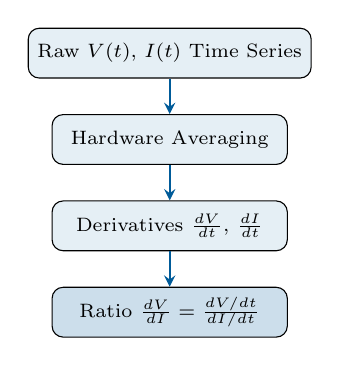
\begin{tikzpicture}[
            box/.style={draw, rectangle, fill=BMEblue!10, text centered, minimum height=1.8em, minimum width=8.5em, rounded corners, font=\scriptsize},
            arrow/.style={-stealth, thick, BMEblue}
        ]
            \node (raw) [box] {Raw $V(t)$, $I(t)$ Time Series};
            \node (filter) [box, below=0.45cm of raw] {Hardware Averaging};
            \node (deriv) [box, below=0.45cm of filter] {Derivatives $\frac{dV}{dt}$, $\frac{dI}{dt}$};
            \node (ratio) [box, below=0.45cm of deriv, fill=BMEblue!20] {Ratio $\frac{dV}{dI} = \frac{dV/dt}{dI/dt}$};
            
            \draw [arrow] (raw) -- (filter);
            \draw [arrow] (filter) -- (deriv);
            \draw [arrow] (deriv) -- (ratio);
        \end{tikzpicture} \\
        \vspace{0.1cm}
        \scriptsize Parametric derivative calculation flow
    \end{columns}
\end{frame}

% =====================================================================
% SECTION 3: QUANTITATIVE RESULTS & CHARACTERIZATION
% =====================================================================
\section{Part 3: Quantitative Results and Characterization}
\begin{frame}[plain,noframenumbering]
    \centering
    \large\bfseries\color{BMEblue}
    Part 3: Quantitative Results and Characterization
\end{frame}

% ---------------------------------------------------------------------
% Slide 8: Single Junction V-I Characteristics
% ---------------------------------------------------------------------
\begin{frame}{Single Junction V-I Characteristics (Task 1)}
    \begin{columns}
        \column{0.5\textwidth}
        \centering
        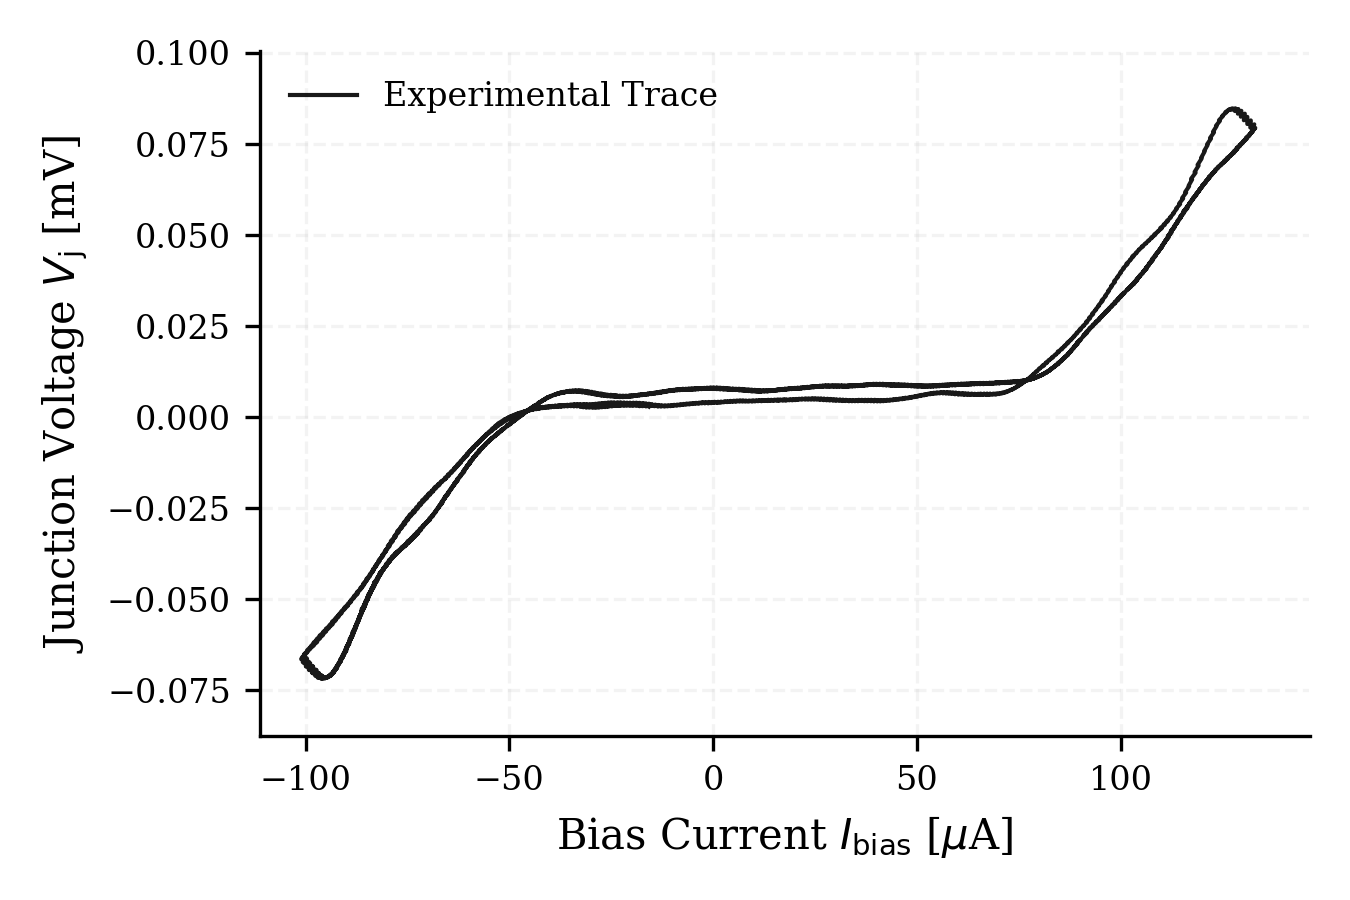
\includegraphics[height=0.55\textheight,keepaspectratio]{task1_iv.png} \\
        \vspace{0.1cm}
        \scriptsize V-I curve driven at $I_{\text{sweep}} = \pm 120\ \mu\text{A} $
        
        \column{0.5\textwidth}
        \textbf{Underdamped Hysteretic Transport} \\
        \vspace{0.2cm}
        The single-junction sweep displays highly stable, hysteretic switching behavior.
        \begin{itemize}
            \item \textbf{Critical Current}: $I_c = 82\ \mu\text{A}$ at the lowest temperature (superconducting threshold).
            \item \textbf{Capacitive Hysteresis}: Hysteretic return path is characteristic of underdamped junctions where capacitance shunting is significant.
            \item \textbf{Gain Validation}: Junction voltage spans $\pm 1.5\text{ mV}$, amplified to $\pm 1.5\text{ V}$ on scope, verifying differential amplifier gain of $1000\times$.
        \end{itemize}
    \end{columns}
\end{frame}

% ---------------------------------------------------------------------
% Slide 9: SQUID Voltage Modulation (Task 2)
% ---------------------------------------------------------------------
\begin{frame}{SQUID Voltage Modulation under Flux Drive (Task 2)}
    \begin{columns}
        \column{0.5\textwidth}
        \centering
        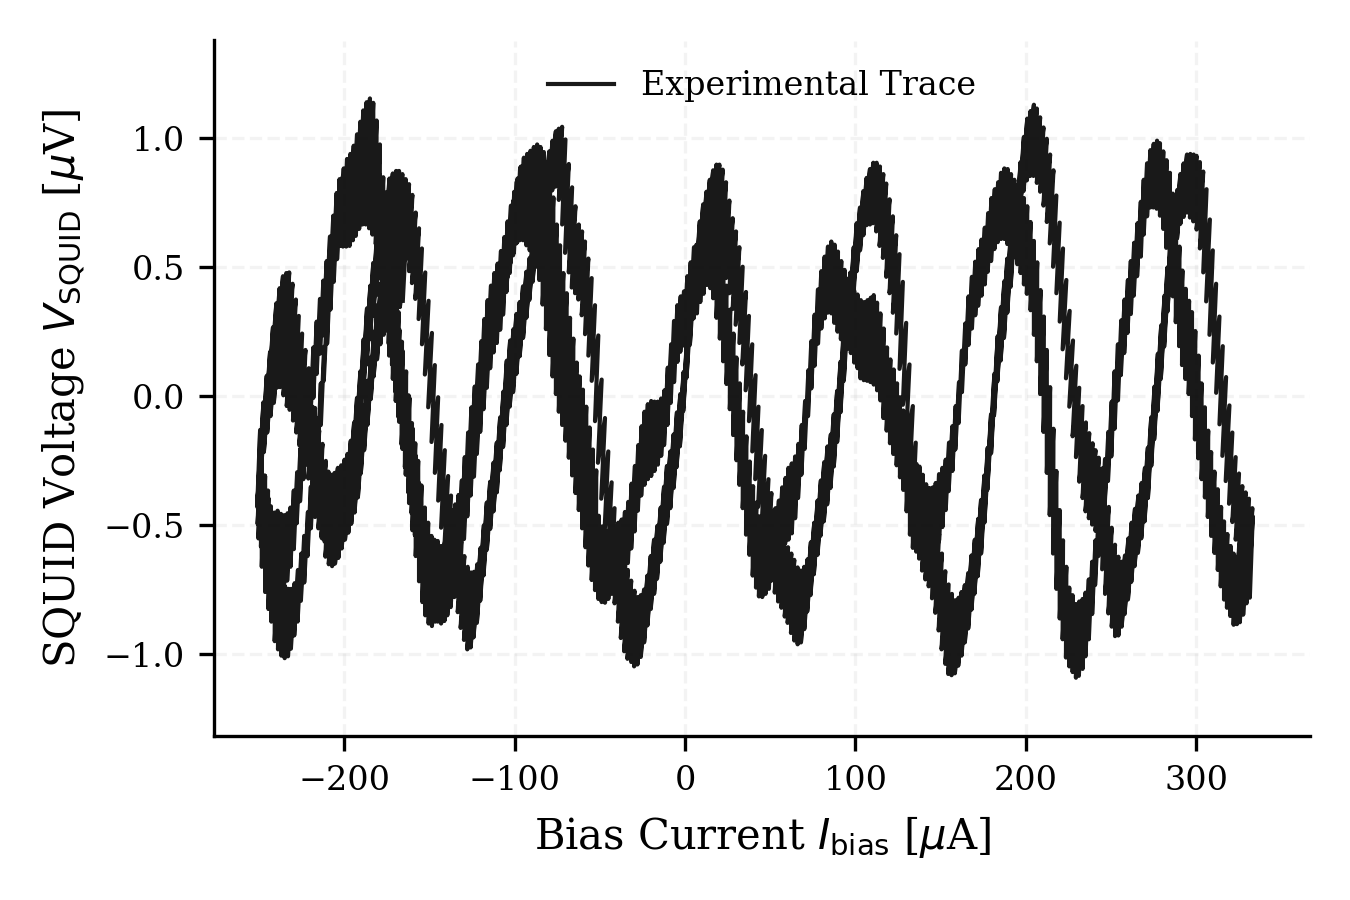
\includegraphics[height=0.55\textheight,keepaspectratio]{task2_iv.png} \\
        \vspace{0.1cm}
        \scriptsize SQUID voltage modulation under 41 Hz triangular flux drive

        \column{0.5\textwidth}
        \textbf{Triangular Flux Sweep} \\
        \vspace{0.2cm}
        We applied a triangular flux-bias current of $\pm 300\ \mu\text{A}$ at a frequency of $41\text{ Hz}$ through the flux line to characterise the SQUID:
        \begin{itemize}
            \item \textbf{Flux Periodicity}: Approximately 6 full flux periods (7 peaks) are clearly resolved within the sweep drive envelope.
            \item \textbf{Stable Cooling}: Confirms robust, stable superconducting phase locking under liquid nitrogen cooling at $77\text{ K}$.
            \item \textbf{V-I Integration}: Demonstrates active voltage-flux transduction $V(\Phi)$ as the basis for magnetometry.
        \end{itemize}
    \end{columns}
\end{frame}

% ---------------------------------------------------------------------
% Slide 10: SQUID Voltage-Flux Transduction & Mutual Inductance (Task 3)
% ---------------------------------------------------------------------
\begin{frame}{SQUID Voltage-Flux Transduction \& Mutual Inductance (Task 3)}
    \begin{columns}
        \column{0.55\textwidth}
        \textbf{Peak-to-Peak Modulation} \\
        \small SQUID voltage oscillates periodically under flux drive:
        \begin{itemize}
            \item Max peak modulation $V_{\text{pp}} = 2.2\ \mu\text{V}$ at DC biases of $1.0\text{ V}$ and $1.1\text{ V}$.
            \item Suppressed to $0.8\ \mu\text{V}$ at $1.5\text{ V}$ bias (normal state).
        \end{itemize}
        
        \vspace{0.1cm}
        \textbf{Mutual Inductance Extraction} \\
        \small Periodicity $\Delta I_{\text{flux}} = 82.9\ \mu\text{A}$ over 14 cycles yields:
        \begin{equation}
            M = \frac{\Phi_0}{\Delta I_{\text{flux}}} = 24.9\text{ pH}
        \end{equation}
        Manual calculation gives $25.2\text{ pH}$ (1.2\% agreement).

        \column{0.45\textwidth}
        \centering
        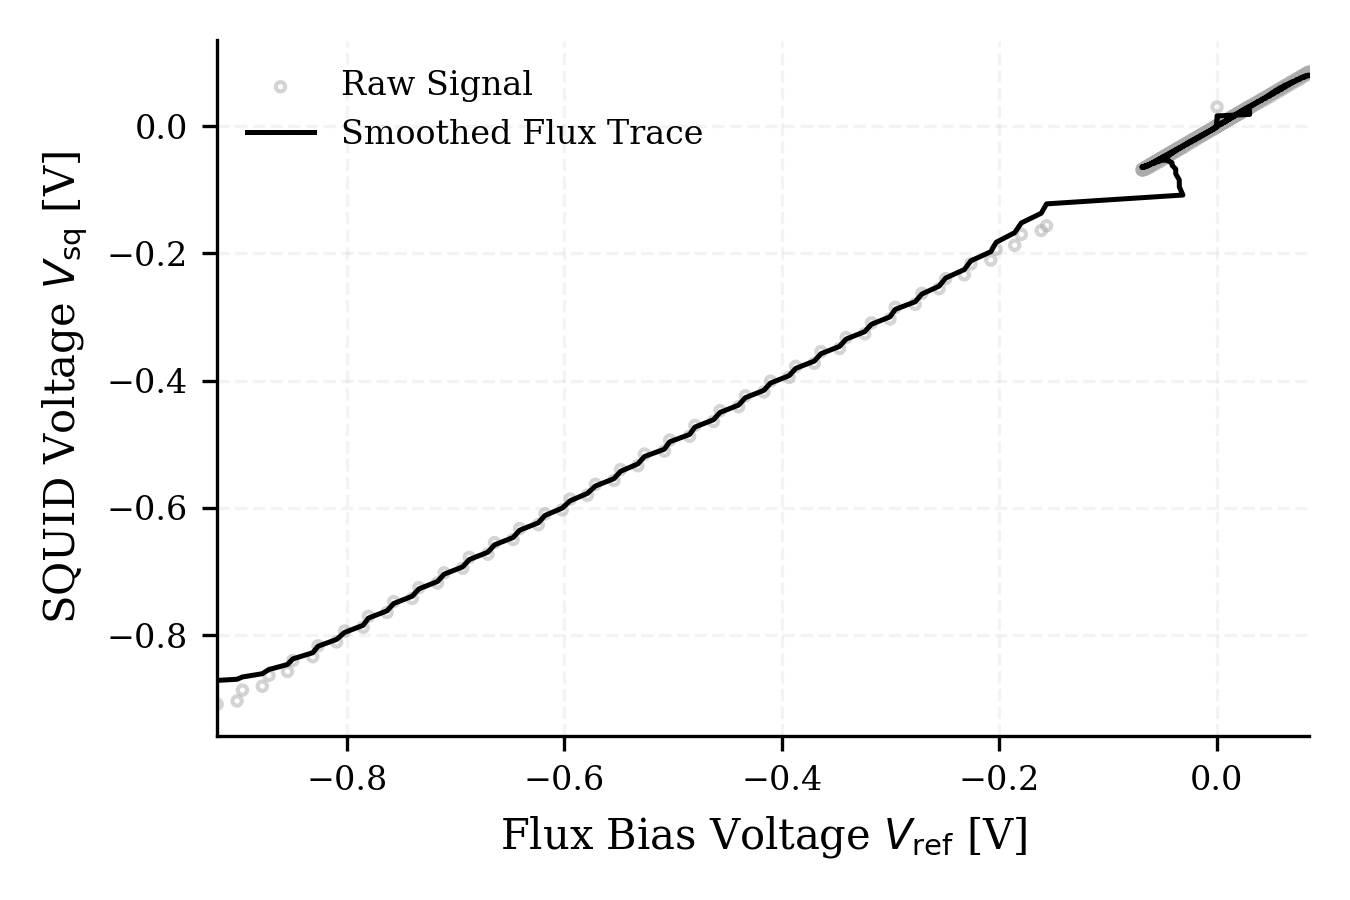
\includegraphics[height=0.52\textheight,keepaspectratio]{task3_flux.png} \\
        \vspace{0.1cm}
        \scriptsize Zoomed SQUID voltage vs. flux bias current
    \end{columns}
\end{frame}

% ---------------------------------------------------------------------
% Slide 10: Critical Current Modulation
% ---------------------------------------------------------------------
\begin{frame}{Critical Current Modulation $I_c(\Phi)$ (Task 3b)}
    \begin{columns}
        \column{0.5\textwidth}
        \centering
        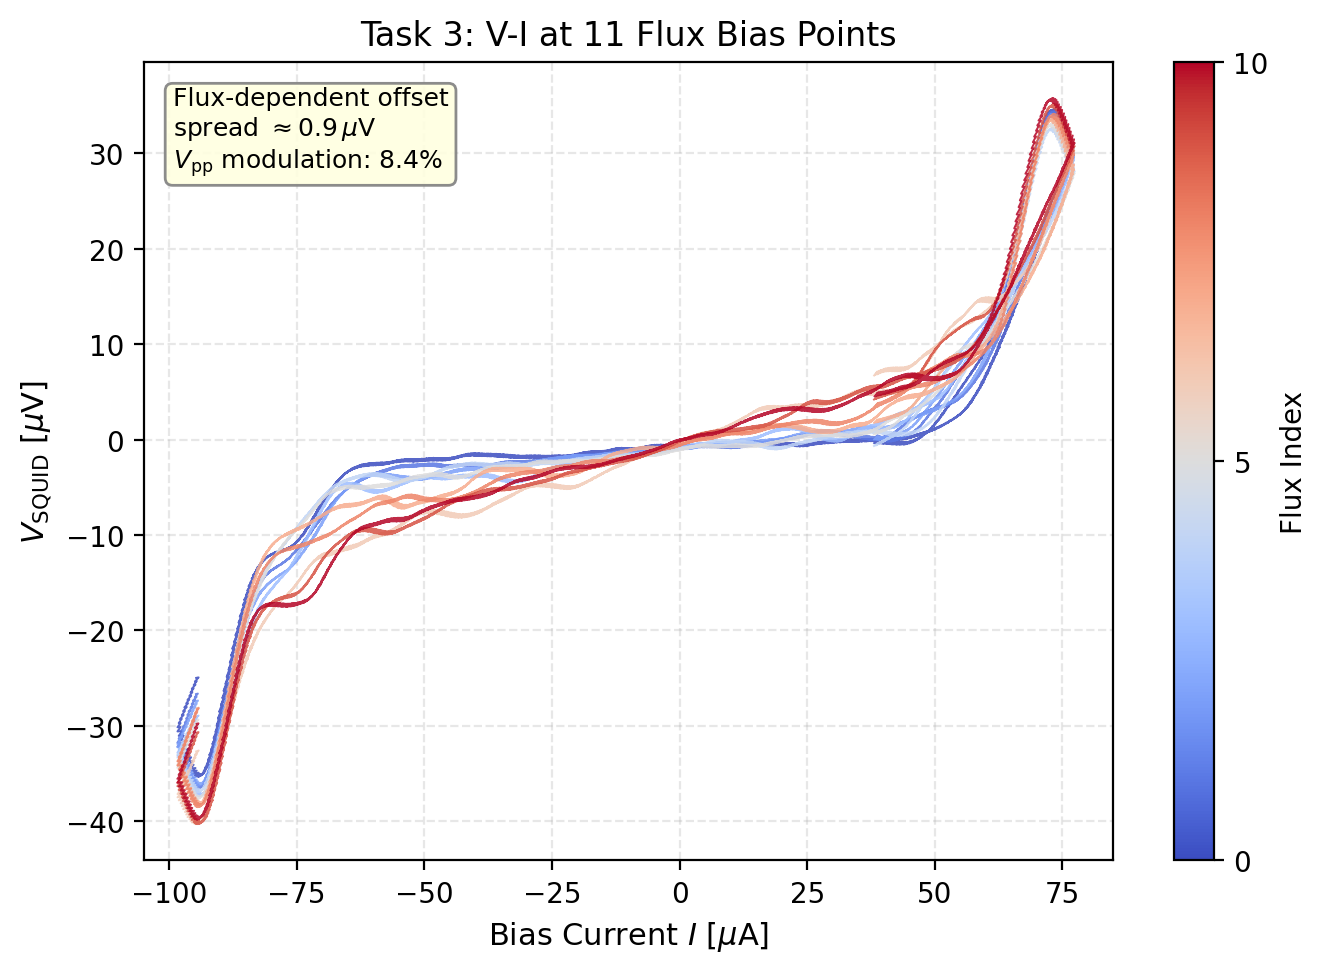
\includegraphics[height=0.55\textheight,keepaspectratio]{../code/task3/task3_flux_vi_overlay.png} \\
        \vspace{0.1cm}
        \scriptsize V-I curves at 11 flux biases spanning one period
        
        \column{0.5\textwidth}
        \textbf{Direct Observation of Quantum Interference} \\
        \vspace{0.2cm}
        V-I curves recorded at 11 flux bias points demonstrate critical current modulation:
        \begin{itemize}
            \item \textbf{Voltage Offset Spread}: $\sim 0.9\ \mu\text{V}$ spread visible near zero current bias.
            \item \textbf{Modulation Depth}: Max modulation depth of $6.0\ \mu\text{V}$ (8.4\% of peak voltage).
            \item \textbf{Phase Tuning}: The continuous transition confirms the macroscopic relation:
            \begin{equation}
                I_{c}(\Phi) = 2I_0\left|\cos\left(\pi\frac{\Phi}{\Phi_0}\right)\right|
            \end{equation}
        \end{itemize}
    \end{columns}
\end{frame}

% =====================================================================
% SECTION 4: SHAPIRO RESONANCES & METROLOGY
% =====================================================================
\section{Part 4: Shapiro Resonances and Advanced Quantum Metrology}
\begin{frame}[plain,noframenumbering]
    \centering
    \large\bfseries\color{BMEblue}
    Part 4: Shapiro Resonances and Advanced Quantum Metrology
\end{frame}

% ---------------------------------------------------------------------
% Slide 11: Phase-Locking under Microwave Irradiation
% ---------------------------------------------------------------------
\begin{frame}{Phase-Locking: AC Josephson Effect}
    \begin{columns}
        \column{0.55\textwidth}
        \textbf{AC Josephson Phase-Locking} \\
        Under microwave irradiation at frequency $\nu$, the external AC field phase-locks the junction's Cooper pair transport, producing constant-voltage plateaus (Shapiro steps) in the V-I curve [Doh et al. 2005].
        
        \vspace{0.3cm}
        \textbf{Quantized Voltage Steps} \\
        \begin{equation}
            \Delta V = n \Phi_0 \nu = n \frac{h}{2e} \nu
        \end{equation}
        For $\nu = 10\text{ GHz}$, the expected fundamental step size is:
        \begin{equation}
            \Delta V_{\text{theory}} = 20.7\ \mu\text{V}
        \end{equation}
        These steps provide the modern, primary physical standard for the definition of the Volt.

        \column{0.45\textwidth}
        \centering
        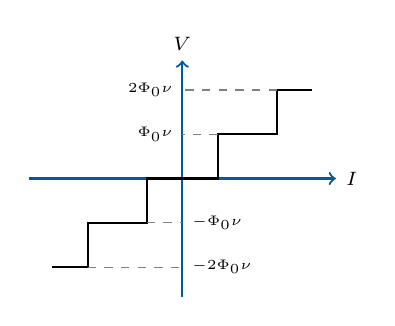
\begin{tikzpicture}[scale=1.5,
            axis/.style={->, thick, BMEblue},
            stepcurve/.style={black, thick}
        ]
            % Axes
            \draw [axis] (-1.3,0) -- (1.3,0) node [right, font=\scriptsize, black] {$I$};
            \draw [axis] (0,-1.0) -- (0,1.0) node [above, font=\scriptsize, black] {$V$};
            
            % Step lines
            \draw [stepcurve] (-1.1,-0.75) -- (-0.8,-0.75) 
                           -- (-0.8,-0.375) -- (-0.3,-0.375) 
                           -- (-0.3,0) -- (0.3,0) 
                           -- (0.3,0.375) -- (0.8,0.375) 
                           -- (0.8,0.75) -- (1.1,0.75);
            
            % Labels on vertical axis
            \draw [dashed, gray] (-0.8,-0.75) -- (0,-0.75) node [right, font=\tiny, black] {$-2\Phi_0\nu$};
            \draw [dashed, gray] (-0.3,-0.375) -- (0,-0.375) node [right, font=\tiny, black] {$-\Phi_0\nu$};
            \draw [dashed, gray] (0.3,0.375) -- (0,0.375) node [left, font=\tiny, black] {$\Phi_0\nu$};
            \draw [dashed, gray] (0.8,0.75) -- (0,0.75) node [left, font=\tiny, black] {$2\Phi_0\nu$};
        \end{tikzpicture} \\
        \vspace{0.1cm}
        \scriptsize Theoretical quantized Shapiro steps staircase
    \end{columns}
\end{frame}

% ---------------------------------------------------------------------
% Slide 12: Step Extraction Methodology - LSCV KDE
% ---------------------------------------------------------------------
\begin{frame}{Step Extraction Methodology: Gaussian LSCV-KDE}
    \begin{columns}
        \column{0.55\textwidth}
        \textbf{Fragility of Ad-hoc Heuristics} \\
        \small Standard $dV/dI$ derivative peak-prominences or histogram bin-widths are highly subjective. At 10 GHz, they yield step estimates ranging wildly from $13.3\ \mu\text{V}$ to $25.6\ \mu\text{V}$ depending on arbitrary tuning parameters.
        
        \vspace{0.1cm}
        \textbf{Least-Squares Cross-Validation (LSCV)} \\
        \small We implement an automated, parameter-free Gaussian Kernel Density Estimator (KDE). LSCV determines the optimal bandwidth $h$ by minimizing:
        \begin{equation}
            \text{LSCV}(h) = \int \hat{f}_h^2 - \frac{2}{N}\sum \hat{f}_{-i,h}(x_i)
        \end{equation}
        \textbf{Central Slicing}: We slice the central 50\% current sweep region to reject normal ohmic branch noise.
        
        \column{0.45\textwidth}
        \textbf{Bandwidth Comparison} \\
        \begin{itemize}
            \item \textbf{Silverman's rule}: $h = 6.7\ \mu\text{V}$ (oversmoothes multimodal peaks, merging plateaus).
            \item \textbf{LSCV optimization}: selects $h = 1.5\ \mu\text{V}$, successfully resolving discrete plateaus spacing of $\sim 20\ \mu\text{V}$ without empirical bias.
        \end{itemize}
    \end{columns}
\end{frame}

% ---------------------------------------------------------------------
% Slide 13: Step Verification at 10 GHz
% ---------------------------------------------------------------------
\begin{frame}{Shapiro Step Verification at 10 GHz (Task 4)}
    \begin{columns}
        \column{0.45\textwidth}
        \textbf{KDE Step Extraction} \\
        \vspace{0.15cm}
        We resolve Shapiro steps using automated Gaussian KDE with LSCV bandwidth optimization:
        \begin{itemize}
            \item \textbf{Peak Resolution}: Resolves 6 symmetric peaks corresponding to step indices $n \in \{-3, -2, -1, 0, +1, +2, +3\}$.
            \item \textbf{High Accuracy}: Median spacing $\Delta V_{\text{KDE}} = 19.7\ \mu\text{V}$, yielding only a \textbf{4.8\% error} against theory ($20.7\ \mu\text{V}$).
            \item \textbf{Objective Selection}: Avoids human bias in step size extraction.
        \end{itemize}

        \column{0.55\textwidth}
        \centering
        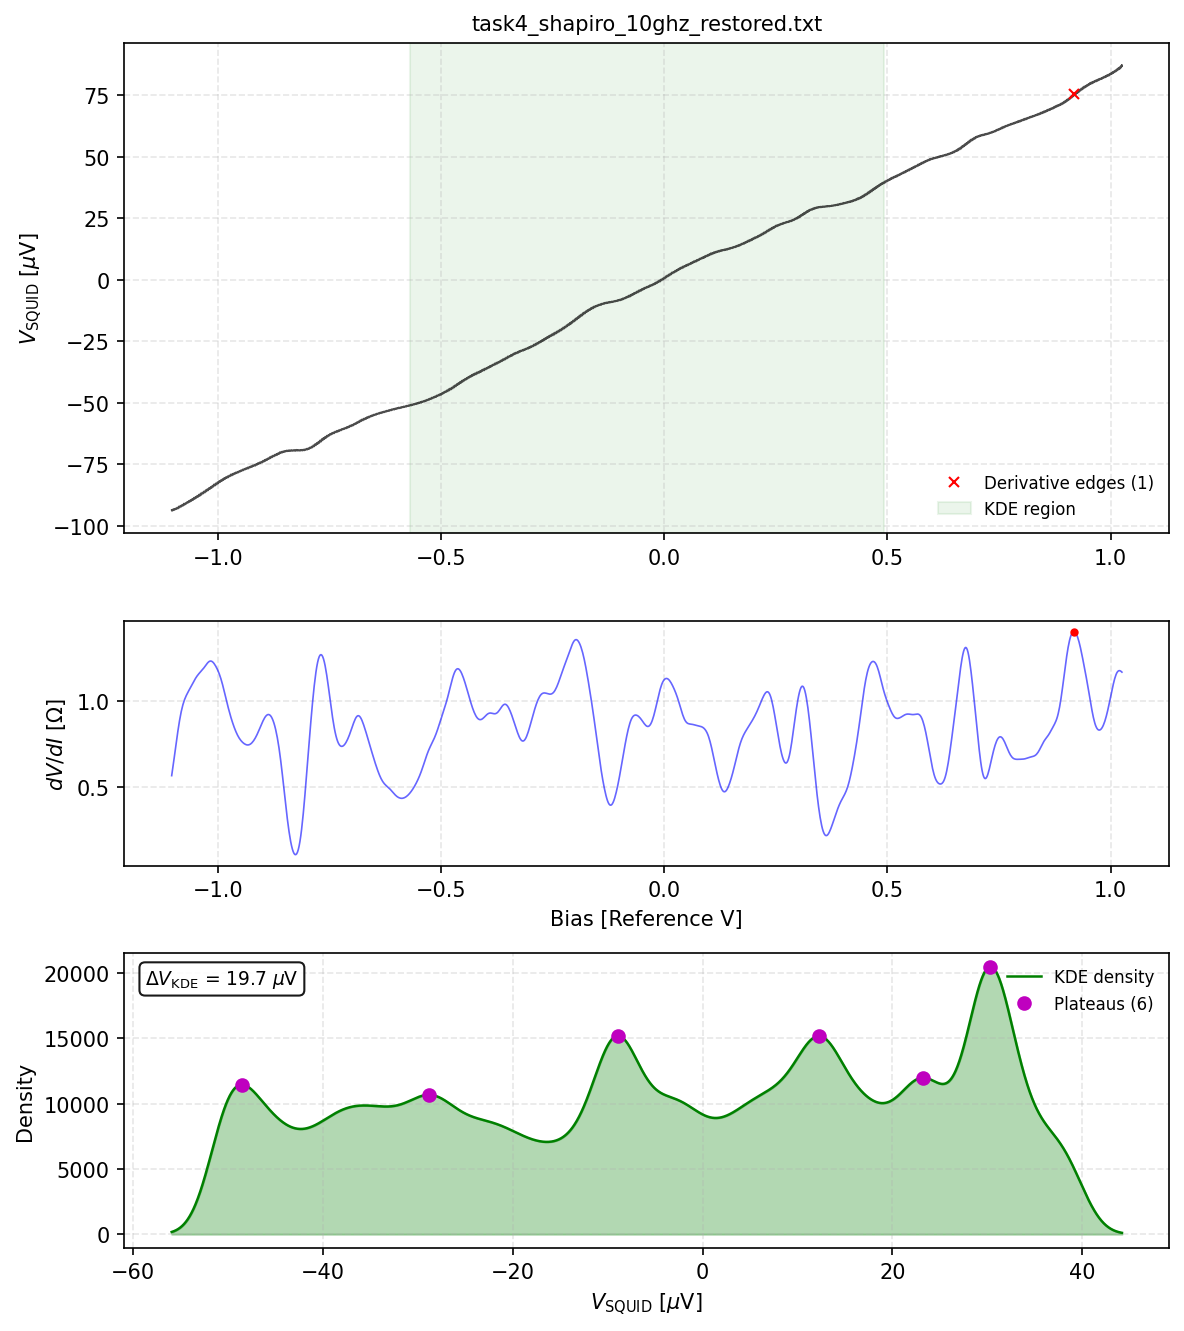
\includegraphics[height=0.70\textheight,keepaspectratio]{../code/task4/task4_shapiro_10ghz_restored_kde_verification.png} \\
        \vspace{0.1cm}
        \scriptsize KDE step extraction workflow at 10 GHz
    \end{columns}
\end{frame}

% ---------------------------------------------------------------------
% Slide 14: Frequency Dependence of Shapiro Steps
% ---------------------------------------------------------------------
\begin{frame}{Frequency Dependence and Bimodal Scattering (Task 5)}
    \begin{columns}
        \column{0.55\textwidth}
        \textbf{Flux Quantum Fitting} \\
        We swept frequency from 8 to 12 GHz. A linear fit through the origin ($\Delta V = \Phi_0 \nu$) yields:
        \begin{equation}
            \Phi_0^{\text{meas}} = 1.71 \times 10^{-15}\text{ Wb}
        \end{equation}
        This represents a 17.3\% deviation from the theoretical value, with an RMSE of $2.7\ \mu\text{V}$.
        
        \vspace{0.2cm}
        \textbf{Standing-Wave Impedance Mismatch} \\
        The data exhibits a bimodal clustering: lower frequencies (8--9.5 GHz) yield step sizes of 12--$15\ \mu\text{V}$, while higher ones (11--12 GHz) cluster at 21--$23\ \mu\text{V}$. 
        
        This physical clustering is a systematic waveguide coupling effect: standing wave resonance on the open SMA line distorts power transfer, rather than a failure of the KDE extractor.
        
        \column{0.45\textwidth}
        \centering
        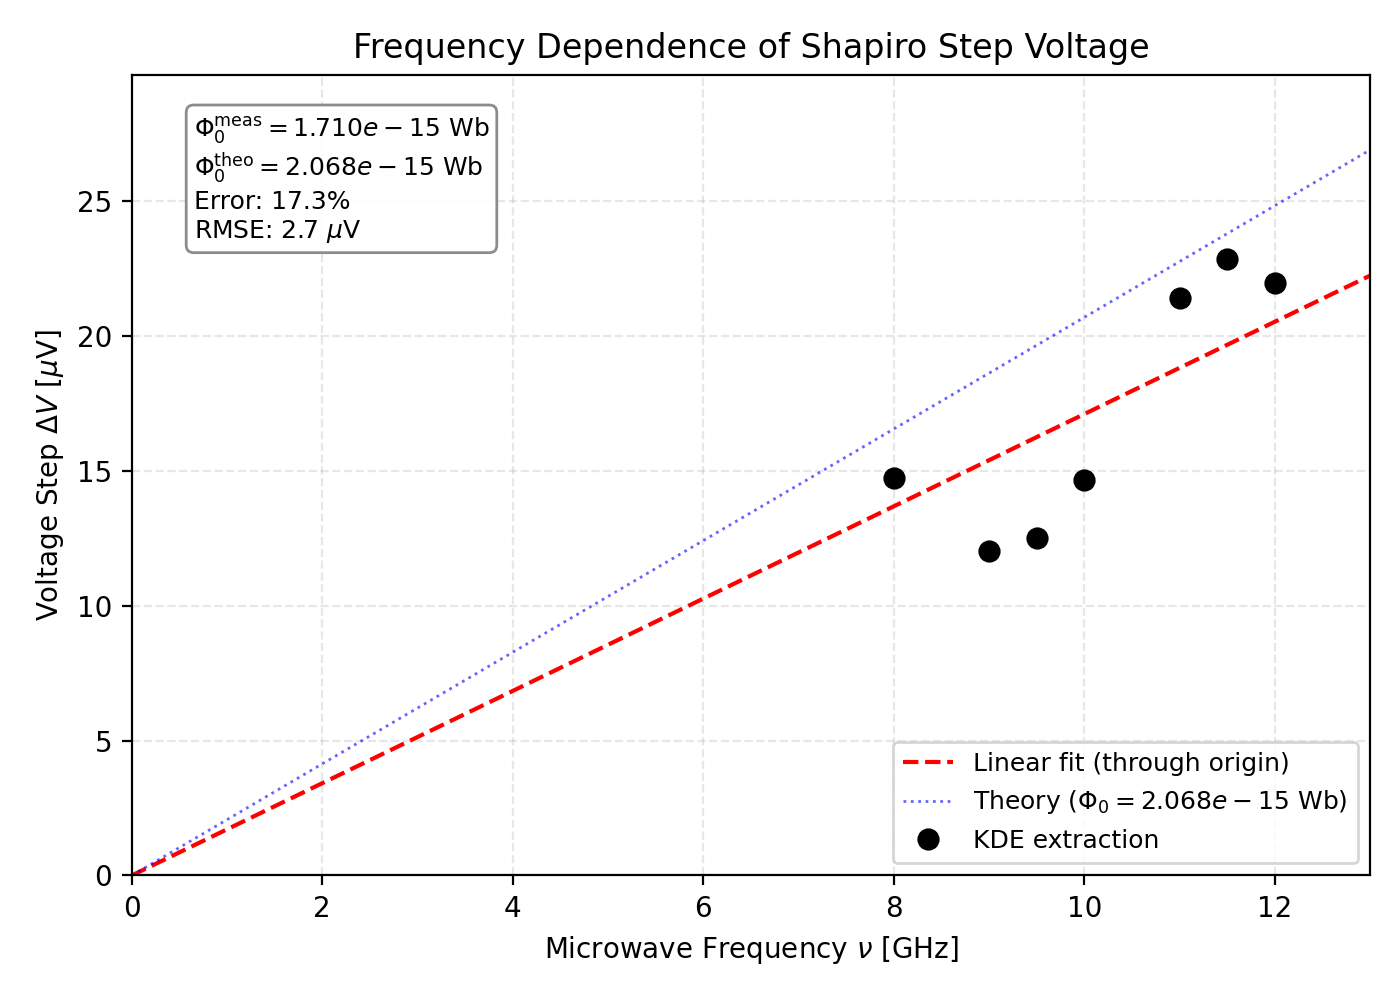
\includegraphics[height=0.52\textheight,keepaspectratio]{../code/task5/task5_frequency_dependence_kde.png} \\
        \vspace{0.1cm}
        \scriptsize Voltage step vs. Frequency
    \end{columns}
\end{frame}

% ---------------------------------------------------------------------
% Slide 15: Power Dependence of Shapiro Steps
% ---------------------------------------------------------------------
\begin{frame}{Power Dependence and Harmonic Steps (Task 6)}
    \begin{columns}
        \column{0.5\textwidth}
        \centering
        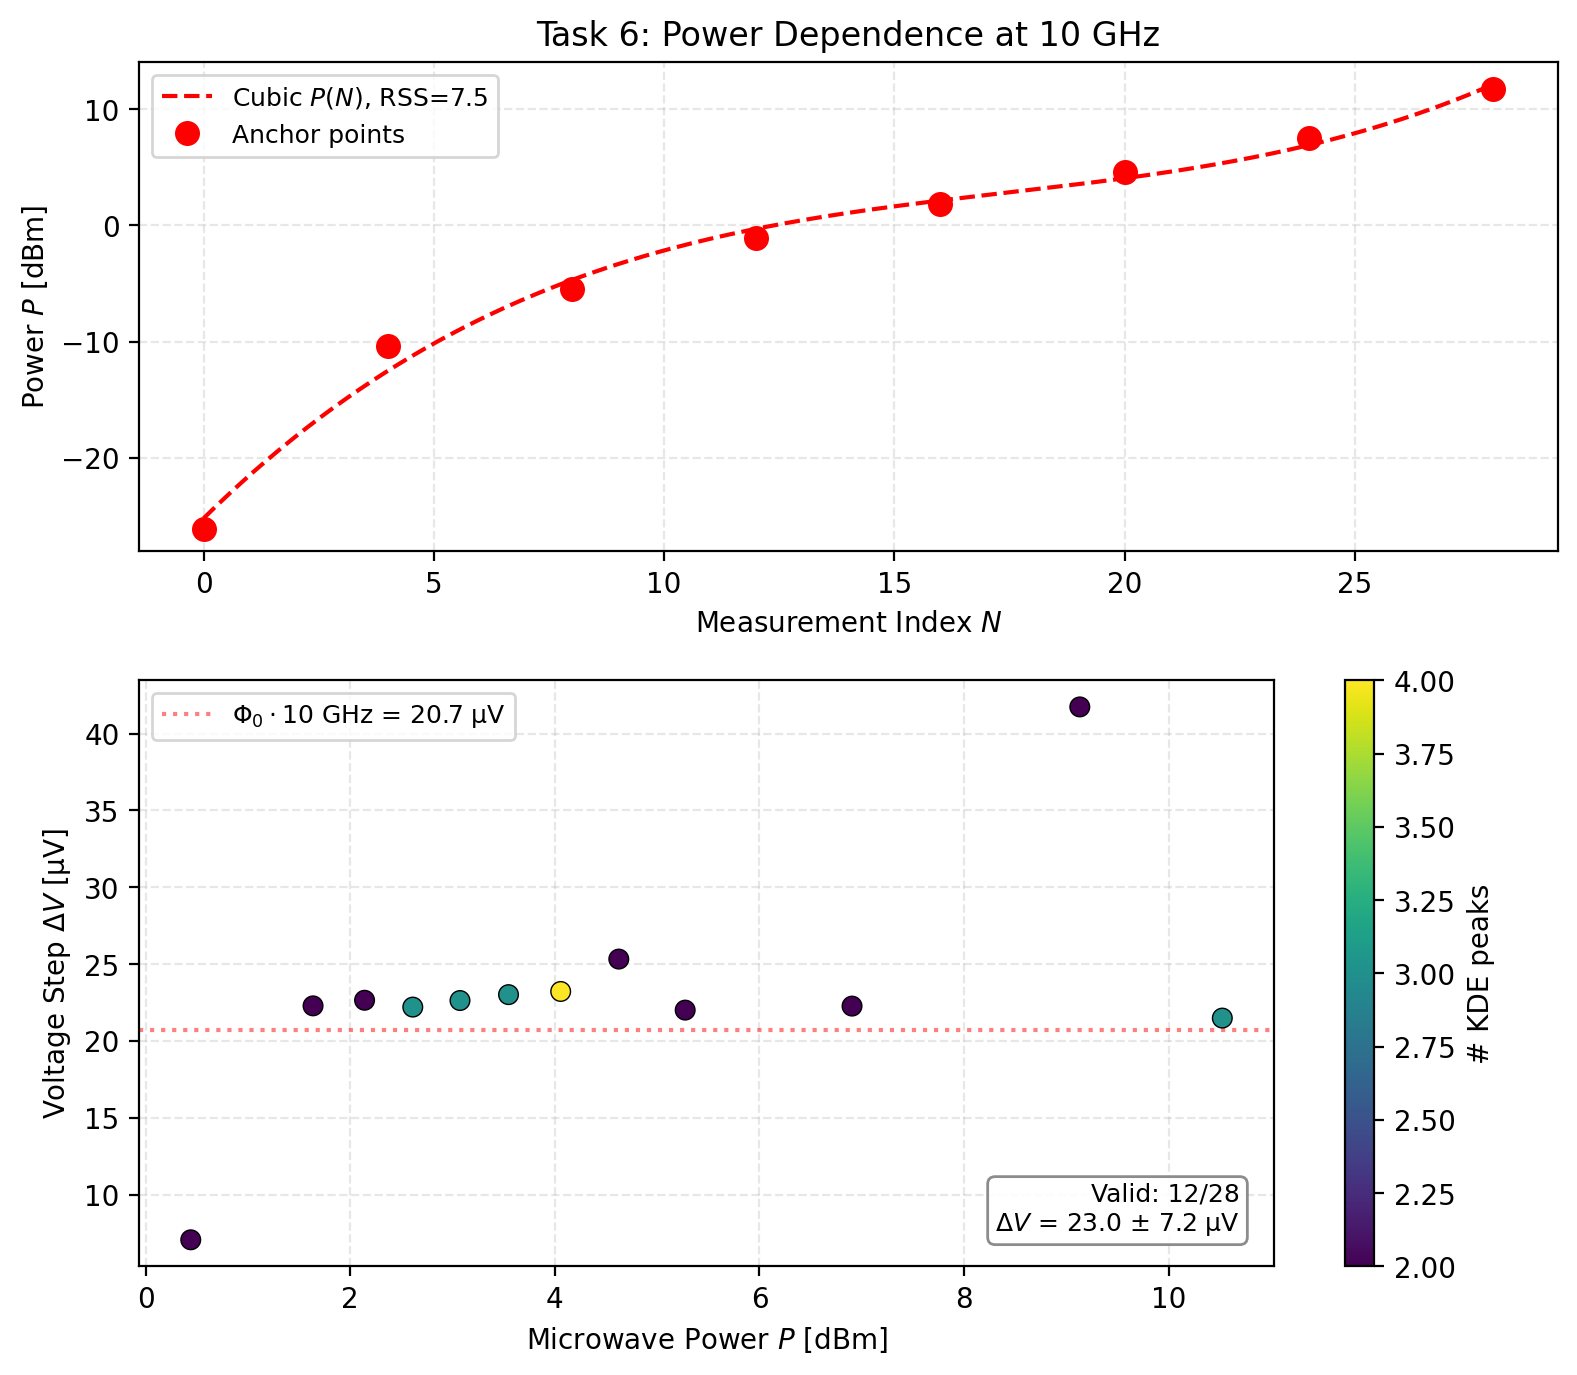
\includegraphics[height=0.55\textheight,keepaspectratio]{../code/task6/task6_power_kde.png} \\
        \vspace{0.1cm}
        \scriptsize Microwave power interpolation and step size vs. power
        
        \column{0.5\textwidth}
        \textbf{Power Sweep \& Interpolation} \\
        \small Sweep markers mapped using a 3rd-order fit:
        $$P(N) = a_3 N^3 + a_2 N^2 + a_1 N + a_0$$
        (RSS = 7.53, parameters $a_i$ stable).
        
        \vspace{0.1cm}
        \textbf{Onset \& Second Harmonic} \\
        \begin{itemize}
            \item \textbf{Threshold}: Steps appear above $\sim 0\text{ dBm}$ ($N > 12$), averaging $\Delta V = 23.0 \pm 7.2\ \mu\text{V}$.
            \item \textbf{Harmonic Step}: Resolved at high power ($9.1\text{ dBm}$): $\Delta V = 41.7\ \mu\text{V} \approx 2 \Delta V_{\text{theory}}$, indicating $n=2$ locking.
        \end{itemize}
    \end{columns}
\end{frame}

% ---------------------------------------------------------------------
% Slide 16: Colormaps of Shapiro Power Sweep
% ---------------------------------------------------------------------
\begin{frame}{Full Spatial Visualization of Shapiro Steps Colormaps}
    \begin{columns}
        \column{0.52\textwidth}
        \centering
        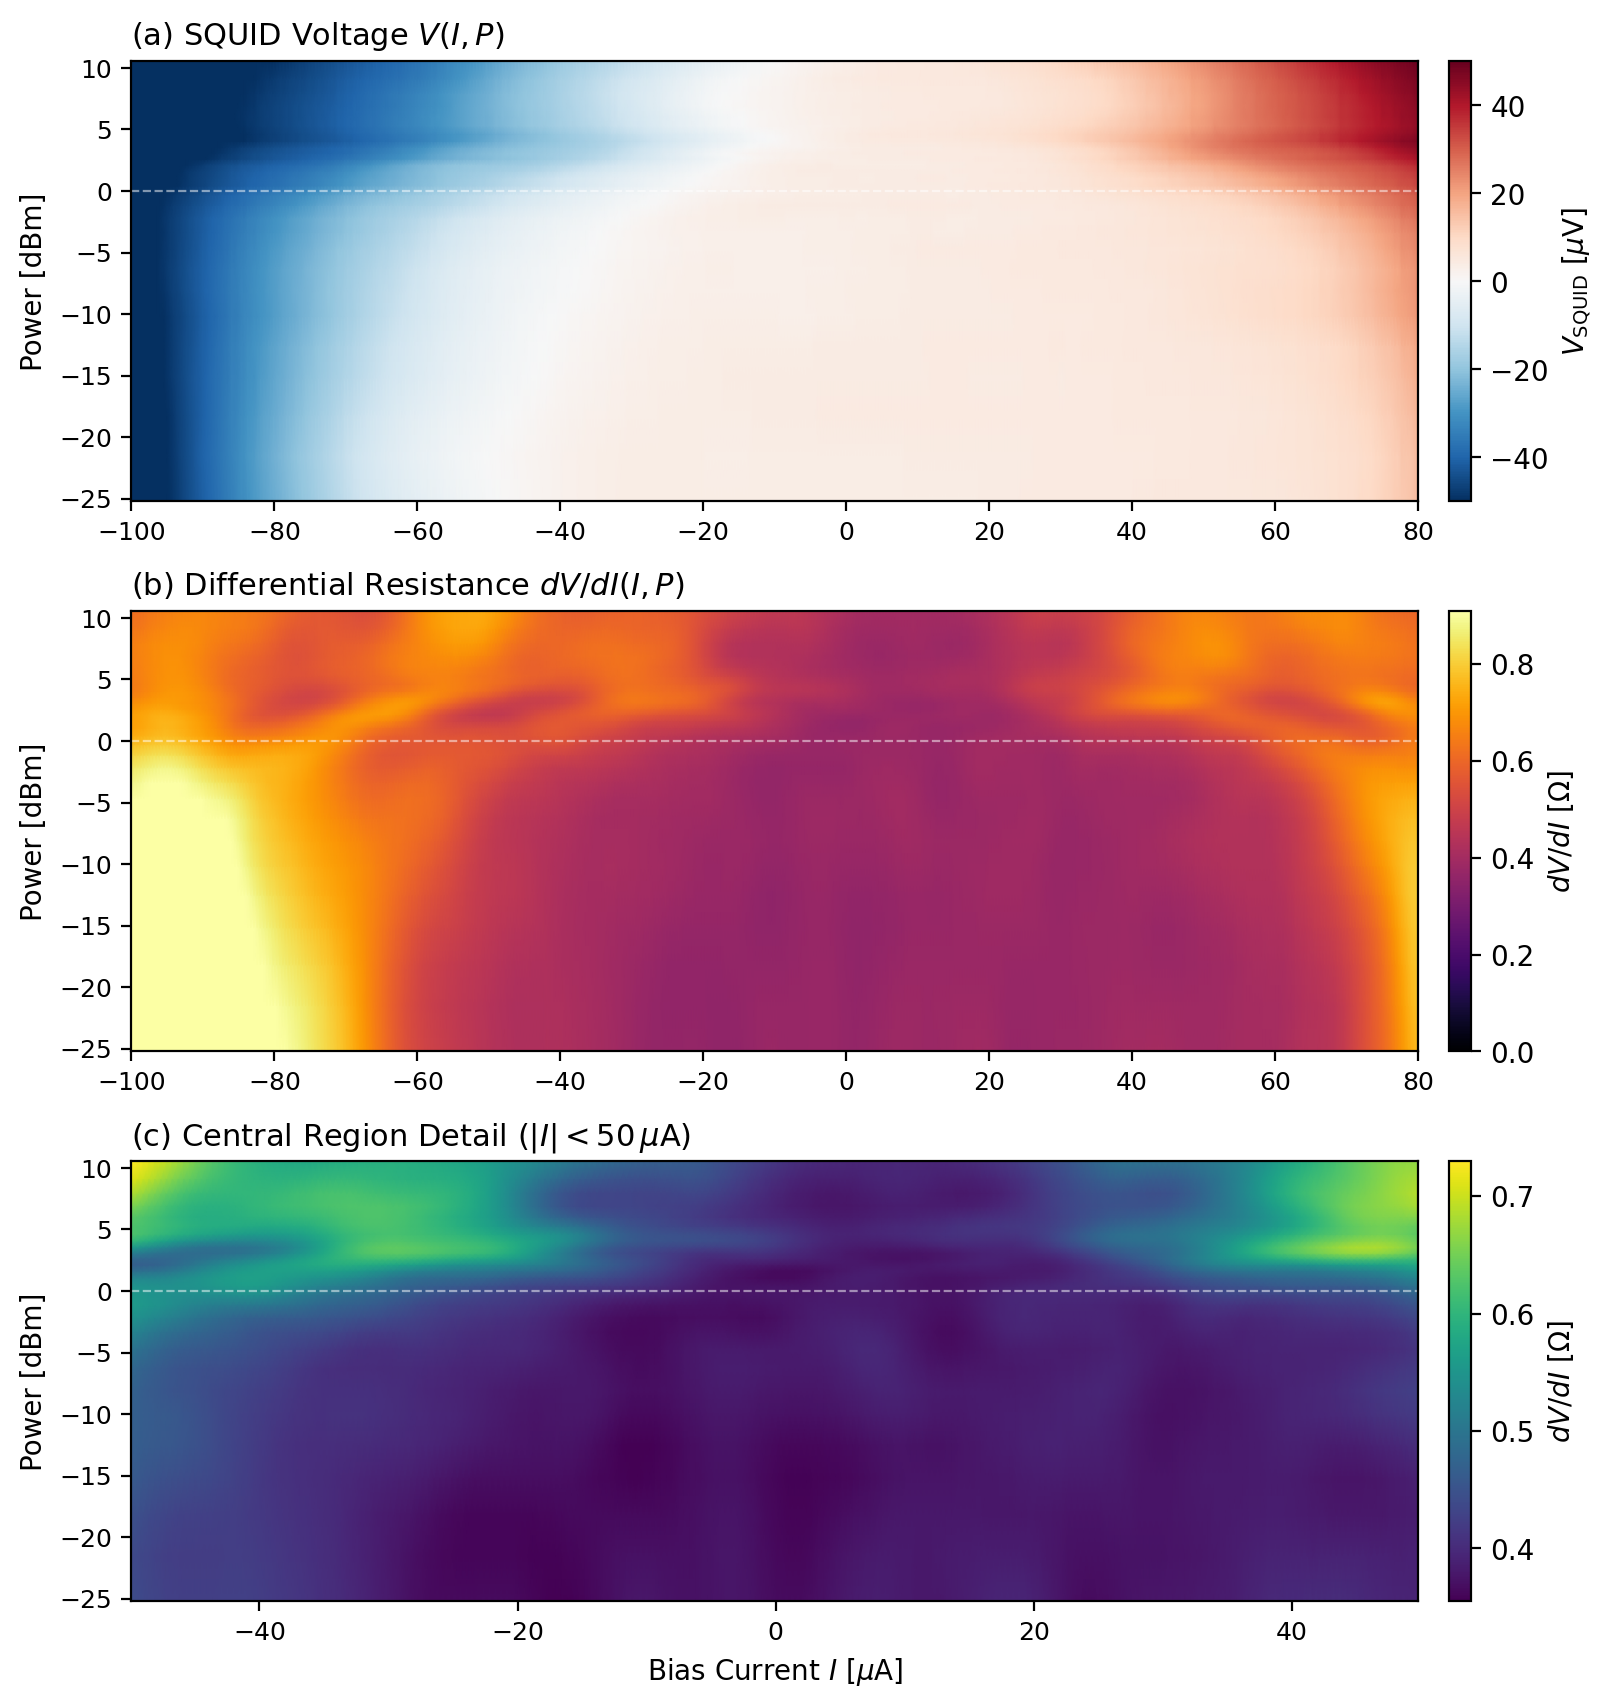
\includegraphics[height=0.75\textheight,keepaspectratio]{../code/task6/task6_colormap.png}
        
        \column{0.48\textwidth}
        \small
        \begin{itemize}
            \item \textbf{Panel (a)} shows the transition broadening of the V-I curves as power increases.
            \vspace{0.2cm}
            \item \textbf{Panel (b)} shows the clear suppression of the critical switching current peaks.
            \vspace{0.2cm}
            \item \textbf{Panel (c)} displays the central region detail, where the emerging structure of Shapiro steps is clearly resolved above $0\text{ dBm}$.
        \end{itemize}
    \end{columns}
\end{frame}

% =====================================================================
% SECTION 5: CONCLUSIONS & OUTLOOK
% =====================================================================
\section{Part 5: Conclusions and Outlook}
\begin{frame}[plain,noframenumbering]
    \centering
    \large\bfseries\color{BMEblue}
    Part 5: Conclusions and Outlook
\end{frame}

% ---------------------------------------------------------------------
% Slide 17: Conclusions
% ---------------------------------------------------------------------
\begin{frame}{Conclusions}
    \textbf{Summary of Achievements} \\
    We completed the comprehensive electrical and quantum characterization of a YBCO DC SQUID at liquid nitrogen temperature ($77\text{ K}$).
    
    \vspace{0.4cm}
    \textbf{Quantitative Findings}:
    \begin{itemize}
        \item \textbf{Junction Transport}: Hysteretic, underdamped V-I trace yielding $I_c = 82\ \mu\text{A}$ at 77K.
        \item \textbf{Flux Magnetometry}: Voltage modulation depth of $2.2\ \mu\text{V}$ yielding $M = 24.9\text{ pH}$ (1.2\% agreement to theory).
        \item \textbf{Quantum Metrology}: Linear voltage steps verified under microwave irradiation. KDE extraction at 10 GHz yields $\Delta V = 19.7\ \mu\text{V}$ (4.8\% error).
        \item \textbf{Physical Verification}: Observed power threshold at $0\text{ dBm}$ and second-harmonic phase locking at $9.1\text{ dBm}$.
    \end{itemize}
    
    \vspace{0.4cm}
    \textbf{Methodology}: Verified that automated Least-Squares Cross-Validation KDE eliminates the subjectivity and large errors of standard ad-hoc peak detection.
\end{frame}

% ---------------------------------------------------------------------
% Slide 18: Outlook & Systematic Challenges
% ---------------------------------------------------------------------
\begin{frame}{Outlook and Systematic Challenges}
    \begin{columns}
        \column{0.55\textwidth}
        \textbf{Impedance Mismatches} \\
        \small Open SMA antenna resonances cause bimodal frequency coupling, yielding 17.3\% error in $\Phi_0$.
        \begin{itemize}
            \item \textbf{PCB Waveguide}: Future designs should employ a matched coplanar waveguide coupler on the SQUID PCB.
        \end{itemize}
        
        \vspace{0.1cm}
        \textbf{Future Improvements} \\
        \begin{itemize}
            \item \textbf{Cryogenic Sensor}: Integrate active temperature sensor to map gap transition $\Delta(T)$.
            \item \textbf{Error Propagation}: Propagate LSCV bandwidth errors directly to the linear fit.
        \end{itemize}

        \column{0.45\textwidth}
        \centering
        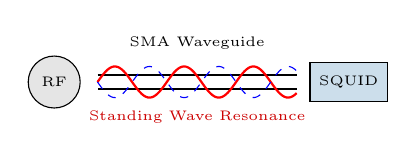
\begin{tikzpicture}[scale=1.1,
            cable/.style={draw, double, double distance=4pt, thick, black},
            junction/.style={draw, fill=BMEblue!20, minimum size=0.5cm},
            wave/.style={draw, red, thick, variable=\x, domain=0:2.3, samples=100}
        ]
            % Cable
            \draw [cable] (0,0) -- (2.3,0);
            \node at (1.15,0.45) [font=\tiny, black] {SMA Waveguide};
            
            % SQUID chip
            \node (sq) at (2.9,0) [draw, rectangle, fill=BMEblue!20, minimum height=0.5cm, font=\tiny] {SQUID};
            % Generator
            \node (gen) at (-0.5,0) [draw, circle, fill=gray!20, minimum size=0.5cm, font=\tiny] {RF};
            
            % Wave representing forward and reflected standing wave
            \draw[red, thick, samples=100] plot[domain=0:2.3] (\x, {0.18*sin(deg(2.5*pi*\x))});
            \draw[blue, dashed, samples=100] plot[domain=0:2.3] (\x, {-0.18*sin(deg(2.5*pi*\x))});
            
            \node at (1.15,-0.4) [red!80!black, font=\tiny] {Standing Wave Resonance};
        \end{tikzpicture} \\
        \vspace{0.1cm}
        \scriptsize SMA cable reflections and power coupling loss
    \end{columns}
\end{frame}

% ---------------------------------------------------------------------
% Slide 19: Acknowledgments
% ---------------------------------------------------------------------
\begin{frame}{Acknowledgments}
    \centering
    \large
    \textbf{We sincerely thank:}
    
    \vspace{0.8cm}
    
    \textbf{Supervisors \& Lab Tutors} \\
    \textit{Oliver Kurtossy, Peter Makk, Szabolcs Csonka, and Andras Halbritter} \\
    For physical guidance and technical sample support.
    
    \vspace{0.5cm}
    
    \textbf{Budapest University of Technology and Economics} \\
    \textit{Department of Physics \& Nanoelectronics Laboratory}
    
    \vspace{0.5cm}
    
    \textbf{Project Framework} \\
    \textit{Practice-Oriented Higher Education Infrastructure and Skills Development at BME} \\
    (Project ID: RRF-2.1.2-21-2022-00005)
\end{frame}

% ---------------------------------------------------------------------
% Slide 20: References
% ---------------------------------------------------------------------
\begin{frame}{References}
    \footnotesize
    \begin{thebibliography}{9}
        \bibitem{solyom} J. S{\'o}lyom, \textit{Fundamentals of the Physics of Solids} (Vol 2), Superconductivity.
        \bibitem{makk} P. Makk, \textit{Transport in complex nanostructures lecture notes}, Josephson Junctions.
        \bibitem{granata} C. Granata et al., ``NanoSQUIDs: Technology and applications'', \textit{Physics Reports}, 614, 1 (2016).
        \bibitem{feynman} \textit{The Feynman Lectures on Physics}, Vol. III, Ch. 21: ``The Schrodinger Equation in a Classical Context''.
        \bibitem{doh} Yong-Joo Doh et al., ``Tunable Supercurrent Through Semiconductor Nanowires'', \textit{Science}, 309, 272 (2005).
        \bibitem{hamalainen} M. H{\"a}m{\"a}l{\"a}inen et al., ``Magnetoencephalography'', \textit{Rev. Mod. Phys.}, 65, 413 (1993).
        \bibitem{vasyukov} D. Vasyukov et al., ``A scanning superconducting quantum interference device with single electron spin sensitivity'', \textit{Nature Nanotechnology}, 8, 639 (2013).
        \bibitem{halbertal} D. Halbertal et al., ``Nanoscale thermal imaging of dissipation in quantum systems'', \textit{Nature}, 539, 407 (2016).
        \bibitem{kalashnikov} D. S. Kalashnikov et al., ``Diode effect in Shapiro steps in an asymmetric SQUID with a superconducting nanobridge'', \textit{Phys. Rev. B}, 112, 144504 (2025).
    \end{thebibliography}
\end{frame}

\end{document}
